\documentclass[a4paper, 14pt]{extarticle}
\usepackage{enumitem}
\usepackage{fefutitle}
\usepackage{xcolor}
\usepackage{amsmath}
\usepackage{graphicx}
\usepackage[justification=centering]{caption}
\usepackage{float}

\begin{document}
	\fefutitle{4}
	\pagebreak	

	\section{Определение цели}
		
	\section{Создание математической модели}
		Математический маятник -- система, состоящая из материальной точки, подвешенной на конце нерастяжимой
		нити. Другой конец нити неподвижен.
		\begin{figure}[H]
			\centering
			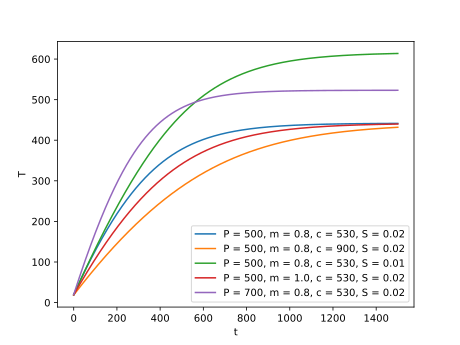
\includegraphics[]{fig1.png}
			\caption[.] {Математический маятник}
		\end{figure}
	
		В записи второго закона Ньютона \(m\vec{a} = \vec{F}\) выделим тангенциальную составляющую
		\(ma_\tau = F_\tau\), получим:
			\[ mL\ddot{\theta} = -mg\sin{\theta}, \]
		где $L$ - длина нити, $\theta$ - угол отклонения маятника, $g$ - ускорение свободного падения 
		$ = 9.8 \text{м/}\text{c}^2)$, $m$ - масса материальной точки
		
		Поделим на $mL$ и перенесём всё в правую часть, \(\dfrac{g}{L} = \omega_0^2 \) - частота собственных
		колебаний:
		\[ \ddot{\theta} + \omega_0^2\sin{\theta} = 0, \]
		
		При малых углах \( \sin{\theta} \approx \theta \) и уравнение превращается в
		\[ \ddot{\theta} + \omega_0^2 \cdot \theta = 0, \]
		
		При наличии затуханий
		\[ \ddot{\theta} + k \dot{\theta} + \omega_0^2\sin{\theta} = 0, \]
		где k - коэффициент затухания
	
	\pagebreak
	\section{Реализация модели}
		Модель была реализована в MathCad.		
		\begin{figure}[H]
			\centering
			\includegraphics[width = \linewidth]{1.jpg}
		\end{figure}
		\begin{figure}[H]
			\centering
			\includegraphics[width = \linewidth]{2.jpg}
		\end{figure}
		\begin{figure}[H]
			\centering
			\includegraphics[width = \linewidth]{3.jpg}
		\end{figure}
		\begin{figure}[H]
			\centering
			\includegraphics[width = \linewidth]{4.jpg}
		\end{figure}
		\begin{figure}[H]
			\centering
			\includegraphics[width = \linewidth]{5.jpg}
		\end{figure}
		\begin{figure}[H]
			\centering
			\includegraphics[width = \linewidth]{6.jpg}
		\end{figure}
		\begin{figure}[H]
			\centering
			\includegraphics[width = \linewidth]{7.jpg}
		\end{figure}
		\begin{figure}[H]
			\centering
			\includegraphics[width = \linewidth]{8.jpg}
		\end{figure}	
		\begin{figure}[H]
			\centering
			\includegraphics[width = \linewidth]{9.jpg}
		\end{figure}
		\begin{figure}[H]
			\centering
			\includegraphics[width = \linewidth]{10.jpg}
		\end{figure}
		\begin{figure}[H]
			\centering
			\includegraphics[width = \linewidth]{11.jpg}
		\end{figure}
		\begin{figure}[H]
			\centering
			\includegraphics[width = \linewidth]{12.jpg}
		\end{figure}
		\begin{figure}[H]
			\centering
			\includegraphics[width = \linewidth]{13.jpg}
		\end{figure}
		\begin{figure}[H]
			\centering
			\includegraphics[width = \linewidth]{14.jpg}
		\end{figure}
		\begin{figure}[H]
			\centering
			\includegraphics[width = \linewidth]{15.jpg}
		\end{figure}
		
	\section{Вывод}
		
		
\end{document}	